% Harmadik előadás

\chapter{Disszipációkezelés}

\section{A disszipációkezelés fontossága}
A processzorok fejlesztésének két iránya van: teljesítmény növelése és a fogyasztás csökkentése.
A fejlesztés fókusza folyamatosan a disszipáció csökkentése felé tolódott, mivel rájöttek, hogy a teljesítmény fő korlátja a disszipáció.

\section{A disszipáció}
A disszipáció két komponensből áll: dinamikus (működés közbeni) és statikus.
A tápegység szempontjából a processzor egy szórt kapacitás, amit a felfutó órajelen fel kell tölteni, a lefutón pedig egy ellenálláson keresztül le kell vezetni.
A töltés-kisülés fogyasztása a dinamikus disszipáció.
A statikus disszipáció a lezárt tranzisztorok szivárgási áramából adódik.
A teljes disszipáció a kettő összege.

\subsection{Kiszámítása}
A dinamikus disszipáció kiszámításához a processzor aktív tranzisztorait egy áramkörrel modellezhetjük (\ref{fig:dyndis}).
\begin{figure}[H]
    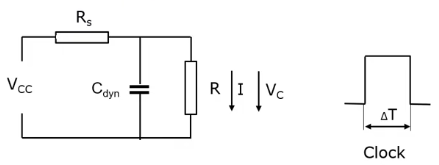
\includegraphics[width=0.8\textwidth]{dyndis}
    \centering
    \caption{Aktív tranzisztorok modellje}
    \label{fig:dyndis}
\end{figure}
Ebből a dinamikus disszipáció kiszámítása:
\begin{equation}
    D_d=2*C_dyn*V_cc^2*f_c
\end{equation}
Az órafrekvenciával lineáris, mivel a töltés-kisülések mennyisége függ tőle.

\section{TDP}
Thermal Design Power, azaz tervezési hőérték.
Egy számításigényes alkalmazás futtatása közbeni maximális disszipációt jelenti.
Fontos, hogy nem teljesen pontos érték.
Az OEM-ek ez alapján tervezik a hűtés rendszereket, aminek legalább ezt a TDP értéket el kell vezetnie úgy, hogy a tranzisztorok hőmérséklete nem megy kb. 80-90°C fölé.
A kategóriák jellemző TDP értékeit mutatja a \ref{fig:tdp}. ábra.
\begin{figure}[H]
    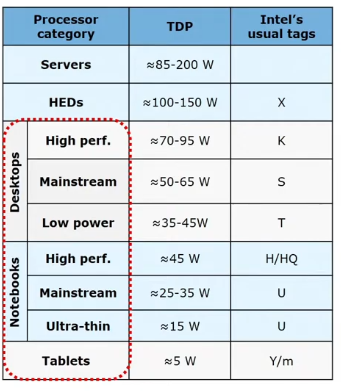
\includegraphics[width=0.6\textwidth]{tdp}
    \centering
    \caption{Processzor osztályok jellemző disszipációja}
    \label{fig:tdp}
\end{figure}
A TDP korlátozza az alapfrekvenciát.
A Turbo működéséhez jóval több watt szükséges.

\section{Intel processzorok disszipációja a fejlődés során}
A \ref{fig:evointel}. ábrán az Intel processzorok lapkamérethez viszonyított disszipációjának növekedése látható az órajel növekedésével.
\begin{figure}[H]
    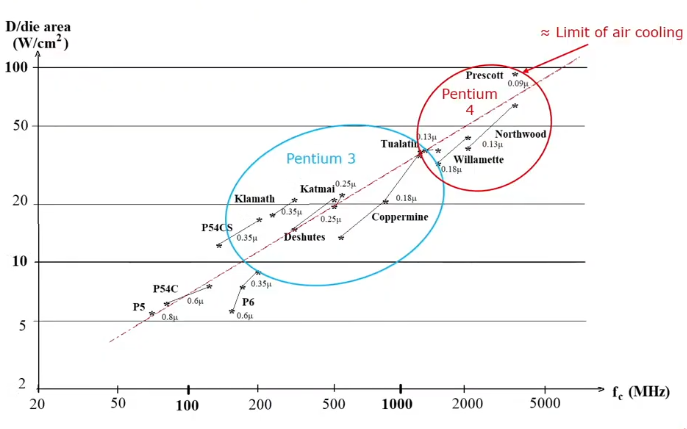
\includegraphics[width=0.8\textwidth]{evointel}
    \centering
    \caption{Disszipáció változása az órajel függvényében}
    \label{fig:evointel}
\end{figure}
Látható, hogy a Pentium 4 Prescott mag már közel 100 wattot adott le cm\textsuperscript{2}-enként, ami a léghűtés fizikai határa.
Az Intel 2000-ben azt várta a Pentium 4 családtól, hogy 10 évig gyártásban marad és 10 GHz órajelet fog elérni.
Ehelyett 2004-ben 4 GHz-nél megakadt a fejlesztés.
A Prescott család bizonyos tagjait kénytelenek voltak visszavonni túlmelegedési problémák miatt.

Ezzel az Intel 2003-tól a nyers teljesítményről áthelyezte a hangsúlyt a teljesítmény per watt, azaz a hatékonyság növelésére.
Összefoglalva a tervezési paradigmák változását mutatja a \ref{fig:paradigm}. ábra.
\begin{figure}[H]
    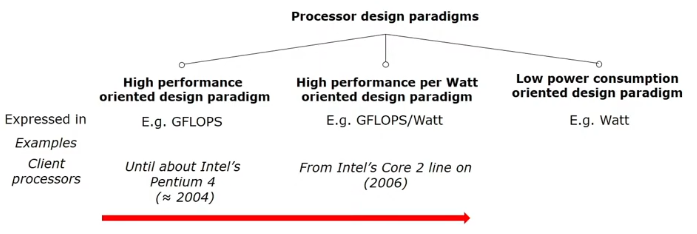
\includegraphics[width=0.8\textwidth]{paradigm}
    \centering
    \caption{Processzor tervezési paradigmák}
    \label{fig:paradigm}
\end{figure}

\section{Disszipációcsökkentő kezdeményezések}
A disszipáció kezelésére megszületett az Energy Star kezdeményezés, az AMD pedig célul tűzte ki, hogy 2014 és 2020 között 20x-osára emeli a hatékonyságot.

\subsection{Energy Star}